\documentclass[11pt]{article}
\usepackage[utf8]{inputenc}
\usepackage[margin=2cm]{geometry}
\usepackage{amsmath, amssymb}
\usepackage{tcolorbox}
\usepackage{float}
\usepackage[colorlinks=true, urlcolor=blue]{hyperref}
\usepackage{tfrupee}
\usepackage{datetime2}
\usepackage{tikz}
\usetikzlibrary{automata, positioning, shapes.multipart, shapes.geometric, arrows.meta, calc}
\begin{document}
\pagestyle{empty}
\hypersetup{
  pdftitle={Design of vending machine controller},
  pdfauthor={Roopesh},
  pdfborderstyle={/S/U/W 1}
}
\begin{center}
  {\Huge Design of vending machine controller}
  \vspace{1em}

  {\small \texttt{Last updated: \today\ \DTMcurrenttime}}
\end{center}
\vspace{1em}
\noindent
\begin{minipage}[t]{0.55\textwidth}
  \section{Design:}
  We have following inputs:
  \begin{itemize}
    \item $X_1$: \rupee 5 inserted
    \item $X_2$: \rupee 10 inserted
  \end{itemize}

  Here we assume input turns 1 when coin is being inserted and 0 when coin has been finished inserting.
  \vspace{1em}

  The state in the system holds current "internal balance" and output. Following are internal balance values:

  \begin{itemize}
    \item 0
    \item 5
    \item 10
    \item $\ge 15$
  \end{itemize}

  \vspace{1.5em}
  {$\ge 15$} value accounts for balance of 15 and 20.

\end{minipage}%
\hfill
\begin{minipage}[t]{0.4\textwidth}
  \vspace{0pt}
  \begin{center}
    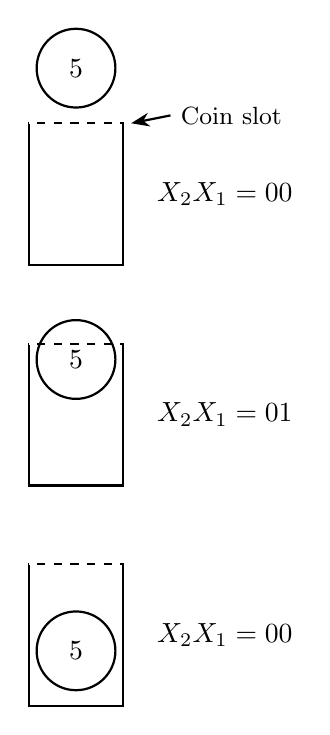
\begin{tikzpicture}[>=Stealth, thick]
      % Sequence 1
      \draw (0,0) rectangle (1.2,1.8);
      \draw (0.6, 2.5) circle (0.5) node {$5$};
      \draw[dashed, white] (0,1.8) -- (1.2,1.8);
      \node[right] at (1.5,0.9) {$X_2X_1 = 00$};
      \draw[<-] (1.3, 1.8) -- (1.8, 1.9) node[right, font=\small] {Coin slot};

      % Sequence 2
      \begin{scope}[yshift=-2.8cm]
        \draw (0,0) rectangle (1.2,1.8);
        \draw[dashed, white] (0,1.8) -- (1.2,1.8);
        \draw (0.6, 1.6) circle (0.5) node {$5$};
        \node[right] at (1.5,0.9) {$X_2X_1 = 01$};
      \end{scope}

      % Sequence 3
      \begin{scope}[yshift=-5.6cm]
        \draw (0,0) rectangle (1.2,1.8);
        \draw[dashed, white] (0,1.8) -- (1.2,1.8);
        \draw (0.6, 0.7) circle (0.5) node {$5$};
        \node[right] at (1.5,0.9) {$X_2X_1 = 00$};
      \end{scope}
    \end{tikzpicture}

    \vspace{1.5em}
    \small Coin insertion sequence and corresponding input.
  \end{center}
\end{minipage}

\section{How state transition occur}

A coin insertion triggers state transition as following: (from initial state)

\vspace{2em}
\begin{center}
  \scalebox{.9}{
    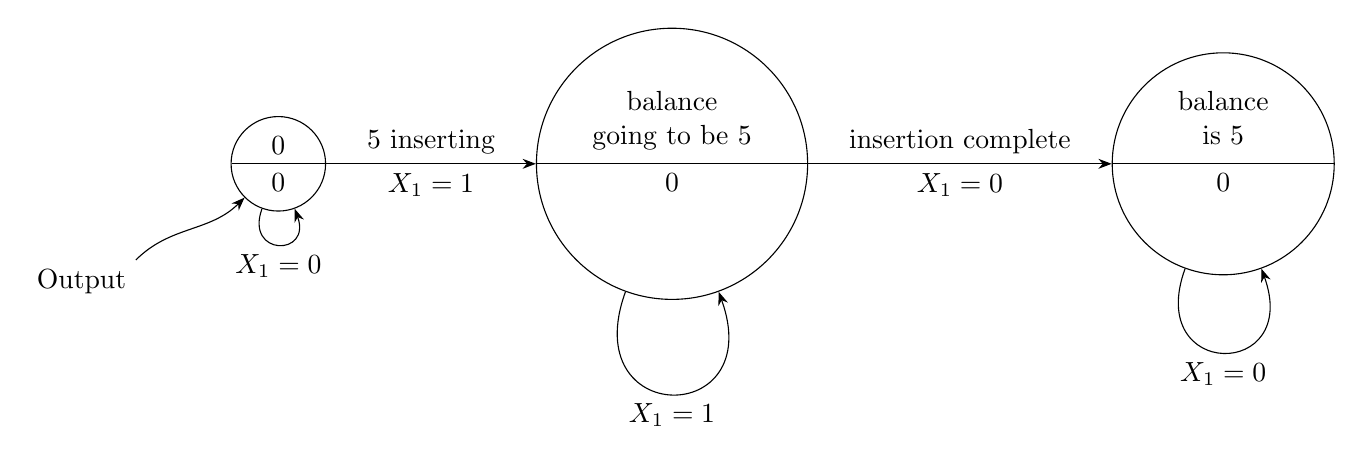
\begin{tikzpicture}[>=Stealth, node distance=4.5cm, auto]
      % State nodes
      \node[circle split, draw, minimum size=1.2cm] (q0) {
        $0$ \nodepart{lower} $0$
      };

      \node[circle split, draw, right of=q0, node distance=5cm] (q1) {
        \begin{tabular}{c} balance \\ going to be 5
        \end{tabular} \nodepart{lower} $0$
      };

      \node[circle split, draw, right of=q1, node distance=7cm, minimum size=1.2cm] (q2) {
        \begin{tabular}{c} balance \\ is 5
        \end{tabular} \nodepart{lower} $0$
      };

      % Transitions

      \draw[->] (q0) -- node[above] {5 inserting} node[below] {$X_1=1$} (q1);
      \path[->] (q0) edge [loop below, out=-110, in=-70, looseness=4] node {$X_1=0$} (q0);

      \path[->] (q1) edge [loop below, out=-110, in=-70, looseness=4] node {$X_1=1$} (q1);

      \draw[->] (q1) -- node[above] {insertion complete} node[below] {$X_1=0$} (q2);
      \path[->] (q2) edge [loop below, out=-110, in=-70, looseness=4] node {$X_1=0$} (q2);

      % Annotation
      \node (output_text) at (-2.5, -1.5) {Output};
      \draw[->, out=45, in=225] (output_text.north east) to (q0.south west);

    \end{tikzpicture}
  }
\end{center}

\vspace{1.5em}
\noindent When coin is being inserted the system goes to a intermediate but stable state (state in the middle shown in figure ). There after when coin is finished inserting it goes to another stable state where internal balance has been incremented (state in rightmost place)

\noindent

\begin{tcolorbox}[colbacktitle=orange, coltitle=black, fonttitle=\large\bfseries, title={Why not directly increment internal balance when coin is being inserted instead of going to a intermediate state?}]

  \noindent You might be tempted to implement this:
  \vspace{.5em}
  \begin{center}
    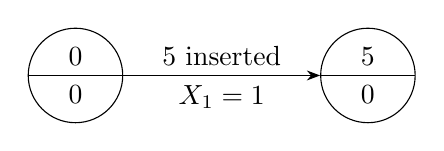
\begin{tikzpicture}[>=Stealth, auto]
      \node[circle split, draw, minimum size=1.2cm] (q0) {
        $0$ \nodepart{lower} $0$
      };
      \node[circle split, draw, right=2.5cm of q0, minimum size=1.2cm] (q1) {
        $5$ \nodepart{lower} $0$
      };

      \draw[->] (q0) -- node[above] {5 inserted} node[below] {$X_1=1$} (q1);
    \end{tikzpicture}
  \end{center}

  \vspace{.5em}
  \noindent It looks like it will works. But in practice this leads to a problem: how long should input be held $1$? If input is held $1$ for too long, the system will quickly traverse through many state in a loop even if input is just a pulse. The below figure shows what happens if $X_1=1$ for a brief period:

  \begin{minipage}[t]{0.5\textwidth}
    \vspace{0pt}
    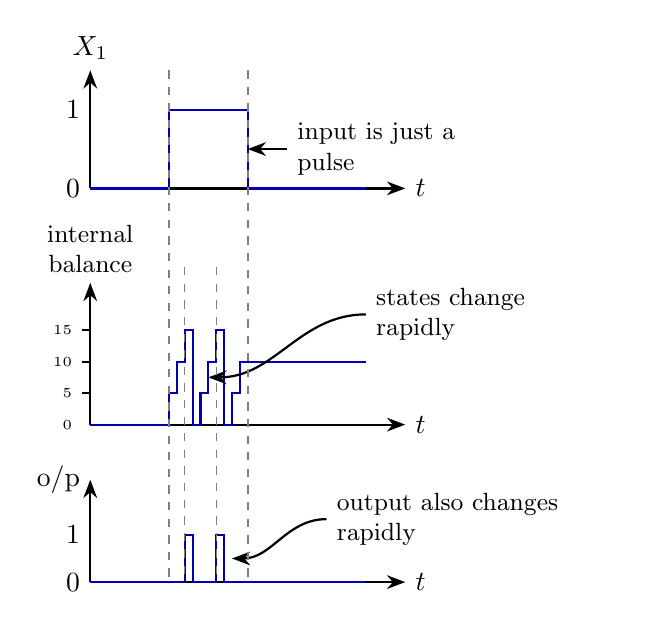
\begin{tikzpicture}[>=Stealth, thick]
      % axes for X1
      \draw[->] (0, 0) -- (4, 0) node[right] {$t$};
      \draw[->] (0, 0) -- (0, 1.5) node[above] {$X_1$};
      \node[left] at (0, 1) {$1$};
      \node[left] at (0, 0) {$0$};

      % X1 pulse
      \draw[blue!70!black, thick] (0,0) -- (1,0) -- (1,1) -- (2,1) -- (2,0) -- (3.5,0);

      % Annotation
      \node[right, font=\small, text width=2cm, align=left] (p_note) at (2.5, 0.5) {input is just a pulse};
      \draw[->] (p_note.west) -- (2, 0.5);

      % axes for internal balance
      \begin{scope}[yshift=-3cm]
        \draw[->] (0, 0) -- (4, 0) node[right] {$t$};
        \node[above, align=center, font=\small] at (0, 1.8) {internal\\balance};
        \draw[->] (0, 0) -- (0, 1.8);
        % ticks
        \foreach \y/\ytext in {0.4/5, 0.8/10, 1.2/15} {
          \draw (-0.1, \y) -- (0, \y) node[left] at (-0.1, \y) {\tiny $\ytext$};
        }
        \node[left] at (-0.1, 0) {\tiny $0$};

        % staircase
        \draw[blue!70!black, thick] (0,0) -- (1,0)
        -- (1,0.4) -- (1.1,0.4)
        -- (1.1,0.8) -- (1.2,0.8)
        -- (1.2,1.2) -- (1.3,1.2)
        -- (1.3,0) -- (1.4,0)
        -- (1.4,0.4) -- (1.5,0.4)
        -- (1.5,0.8) -- (1.6,0.8)
        -- (1.6,1.2) -- (1.7,1.2)
        -- (1.7,0) -- (1.8,0)
        -- (1.8,0.4) -- (1.9,0.4)
        -- (1.9,0.8) -- (3.5,0.8); % matching the end of the pulse

        % Annotation
        \node[right, font=\small, text width=3cm, align=left] (s_note) at (3.5, 1.4) {states change\\rapidly};
        \draw[->] (s_note.west) to[out=180, in=0] (1.5, 0.6);
      \end{scope}

      % axes for o/p
      \begin{scope}[yshift=-5cm]
        \draw[->] (0, 0) -- (4, 0) node[right] {$t$};
        \draw[->] (0, 0) -- (0, 1.3) node[left] {o/p};
        \node[left] at (0, 0.6) {$1$};
        \node[left] at (0, 0) {$0$};
        % output pulses
        \draw[blue!70!black, thick] (0,0) -- (1.2,0)
        -- (1.2,0.6) -- (1.3,0.6)
        -- (1.3,0) -- (1.6,0)
        -- (1.6,0.6) -- (1.7,0.6)
        -- (1.7,0) -- (3.5,0);

        % Annotation
        \node[right, font=\small, text width=3.5cm, align=left] (o_note) at (3, 0.8) {output also changes\\rapidly};
        \draw[->] (o_note.west) to[out=180, in=0] (1.8, 0.3);
      \end{scope}

      % Vertical alignment lines
      \draw[dashed, gray] (1, 1.5) -- (1, -5);
      \draw[dashed, gray, thin] (1.2, -1.0) -- (1.2, -5);
      \draw[dashed, gray, thin] (1.6, -1.0) -- (1.6, -5);
      \draw[dashed, gray] (2, 1.5) -- (2, -5);

    \end{tikzpicture}
  \end{minipage}%
  \hfill
  \begin{minipage}[t]{0.48\textwidth}
    \vspace{4.5em}
    \begin{center}
      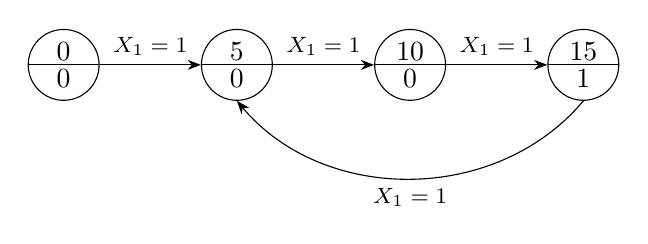
\begin{tikzpicture}[>=Stealth, auto]
        \node[circle split, draw, inner sep=1.5pt, minimum size=0.9cm] (q0) at (0,0) {$0$ \nodepart{lower} $0$};
        \node[circle split, draw, inner sep=1.5pt, minimum size=0.9cm] (q1) at (2.2,0) {$5$ \nodepart{lower} $0$};
        \node[circle split, draw, inner sep=1.5pt, minimum size=0.9cm] (q2) at (4.4,0) {$10$ \nodepart{lower} $0$};
        \node[circle split, draw, inner sep=1.5pt, minimum size=0.9cm] (q3) at (6.6,0) {$15$ \nodepart{lower} $1$};

        \draw[->] (q0) -- node[above, font=\footnotesize] {$X_1=1$} (q1);
        \draw[->] (q1) -- node[above, font=\footnotesize] {$X_1=1$} (q2);
        \draw[->] (q2) -- node[above, font=\footnotesize] {$X_1=1$} (q3);

        \draw[->] (q3.south) to[bend left=50] node[below, font=\footnotesize] {$X_1=1$} (q1.south);
      \end{tikzpicture}
    \end{center}
  \end{minipage}

  \vspace{1em}
  \noindent The internal state quickly switches as fast the circuit allows, hence all states become unstable when input becomes 1.
\end{tcolorbox}

\section{State Diagram \& Flow table}

We define states as following:
\begin{itemize}
  \item $A$: intital state, balance = 0 (output = 0)
  \item $B$: balance is going to be 5 (output = 0)
  \item $C$: balance is 5 (output = 0)
  \item $D$: balance is going to be 10 (output = 0)
  \item $E$: balance is 10 (output = 0)
  \item $F$: balance is going to be $\ge 15$ (output = 0)
  \item $G$: balance is $\ge 15$ (output = 1)
\end{itemize}

When state $G$ has reached, the vending machine dispenses. From $G$ the state transition scheme is as following: if input is 5, it goes to $B$ and if input is $10$ it goes to $C$.
\begin{tcolorbox}[fonttitle=\large\bfseries, title={But in question it is told that the state to be reset to initial state after dispensing?}]
  Indeed in question it is told that the state to be reset to 0. But since we are implementing a Moore machine, we cant do that directly. Because again the problem rises: what input should drive system to go from $G$ to $A$ while keeping the output stable for a while? This can be done only with Mealy machine where output depends on input and present state. However as you can guess, K-map simplification and circuit implementation will become very complex for output variable. Hence that requirement is carefully ignored. (This doesnt affect the overall functionality of vening machine).

\end{tcolorbox}


Based on this we can arrive at following state diagram and Flow table.

\vspace{1em}
\begin{minipage}{.6\textwidth}
\begin{center}
\hspace{-1cm}
\resizebox{\linewidth}{!}{
  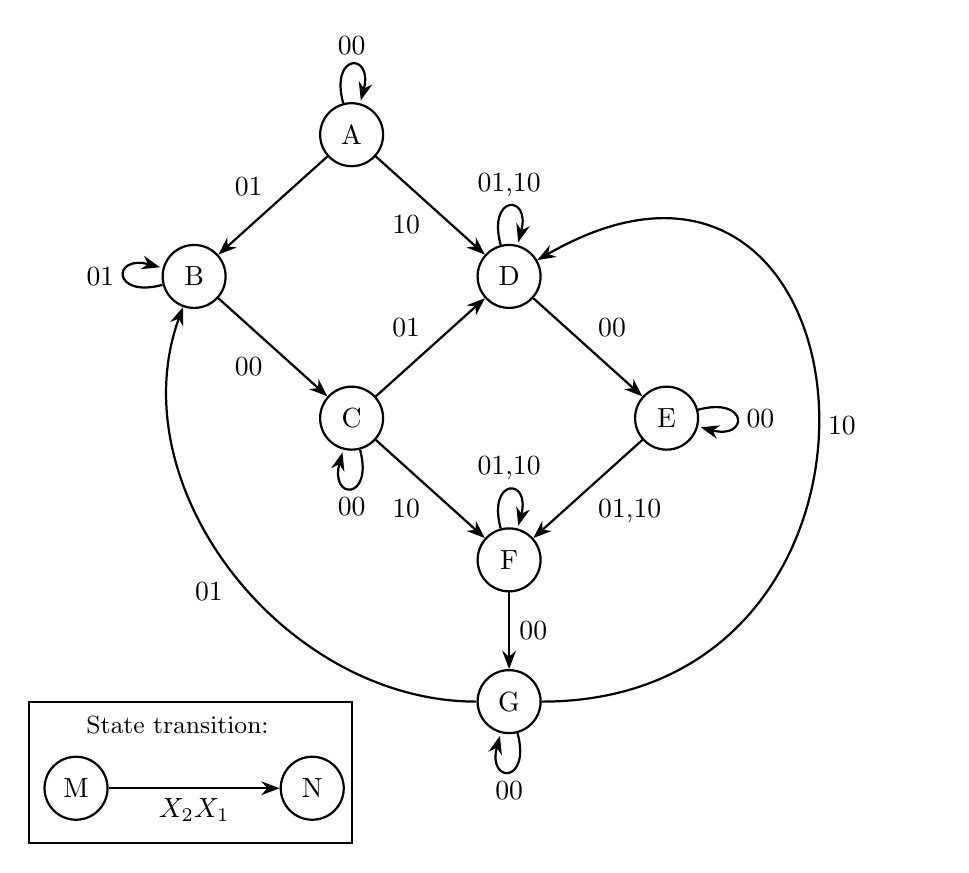
\begin{tikzpicture}[>=Stealth, thick,
    state/.style={circle, draw, minimum size=0.8cm, inner sep=2pt}]
    % Nodes
    \node[state] (A) at (0, 0) {A};
    \node[state] (B) at (-2, -1.8) {B};
    \node[state] (D) at (2, -1.8) {D};
    \node[state] (C) at (0, -3.6) {C};
    \node[state] (E) at (4, -3.6) {E};
    \node[state] (F) at (2, -5.4) {F};
    \node[state] (G) at (2, -7.2) {G};

    % Loops
    \path[->] (A) edge [loop above] node {00} (A);
    \path[->] (B) edge [loop left] node {01} (B);
    \path[->] (D) edge [loop above] node {01,10} (D);
    \path[->] (C) edge [loop below] node {00} (C);
    \path[->] (E) edge [loop right] node {00} (E);
    \path[->] (F) edge [loop above] node {01,10} (F);
    \path[->] (G) edge [loop below] node {00} (G);

    % Edges
    \draw[->] (A) -- node[above left] {01} (B);
    \draw[->] (A) -- node[below left] {10} (D);
    \draw[->] (B) -- node[below left] {00} (C);
    \draw[->] (C) -- node[above left] {01} (D);
    \draw[->] (C) -- node[below left] {10} (F);
    \draw[->] (D) -- node[above right] {00} (E);
    \draw[->] (E) -- node[below right] {01,10} (F);
    \draw[->] (F) -- node[right] {00} (G);


    % Curved lines
    \draw[->] (G) to[out=180, in=250, looseness=1] node[below left] {01} (B);
    \draw[->] (G) to[out=0, in=390, looseness=2.3] node[below right] {10} (D);
    \begin{scope}[yshift=-7.5cm, xshift=-3.5cm]
        \node[state] (M) at (0, -.8) {M};
        \node[state] (N) at (3, -.8) {N};
        \draw[->] (M) -- node[below] {$X_2X_1$} (N);
        \node[right, font=\small, text width=3cm, align=left] (s_note) at (0, 0) {State transition:};
        \draw (-.6, .3) rectangle (3.5, -1.5);
    \end{scope}
  \end{tikzpicture}
  }
  \vspace{1em}
  {\bfseries \large {State diagram}}
\end{center}
\end{minipage}
\hspace{-1cm}
\begin{minipage}{.4\textwidth}
\begin{center}
\resizebox{\linewidth}{!}{
  \renewcommand{\arraystretch}{1.3}
  \begin{tabular}{|c|c|c|c|c|}
    \hline
    \textbf{Present State} & \multicolumn{4}{c|}{\textbf{Input $X_2X_1$}} \\ \cline{2-5}
    & \textbf{00} & \textbf{01} & \textbf{10} & \textbf{11} \\ \hline
    A & A, 0 & B, \_ & D, \_   & \_,\_ \\ \hline
    B & C, \_ & B, 0 & \_, \_ & \_,\_ \\ \hline
    C & C, 0 & D, \_ & F, \_   & \_,\_ \\ \hline
    D & E, \_ & D, 0 & D, 0   & \_,\_ \\ \hline
    E & E, 0 & F, \_ & F, \_   & \_,\_ \\ \hline
    F & G, \_ & F, 0 & F, 0   & \_,\_ \\ \hline
    G & G, 1 & B, \_ & D, \_   & \_,\_ \\ \hline
  \end{tabular}
}

\vspace{1em}
{\bfseries \large {Flow table}}

\end{center}
\end{minipage}
\vspace{1em}

\subsection*{Explanation:}

\begin{enumerate}
\item Initally system is at state $A$.
\item When a \rupee 5 is inserted the state becomes to $B$ (as it indicates "balance is going to be \rupee 5") and if \rupee 10 was inserted the state goes to $D$ (indicating "balance is going to be \rupee 10").
\item After coin has been finished inserting ($X_2X_1=00$) the system can go from $B$ to $C$ (that is "balence \emph{is} 5" state). And it can only go to $C$ as at that time only \rupee 5 is being inserted and no other coin can be inserted simultaneously (hence transition $X_2X_1=10$ is not drawn from $B$ and is considered don't care in flow table.)
\item From $C$, system goes to $D$ if \rupee 5 is inserted (as $D$ indicates "balance is going to be 10") and if \rupee 10 is inserted it goes to $F$ (balance is going to be $\ge$ \rupee 15).
\item From $D$, system goes to $E$ (balance \emph{is} \rupee 10) when either of the coin has finished inserting ($X_2X_1=00$).
\item From $E$ system goes $F$ if any of the coin is being inserted.
\item From $F$ system goes to $G$ (balance \emph{is} $\ge$ \rupee 15) and output $z=1$. This is the only state where output becomes 1.
\item From $G$ system goes to $B$ if \rupee 5 is being inserted and it goes to $D$ if \rupee 10 is being inserted.
\end{enumerate}
State reduction is not done here, as each state already have a definite meaning, reducing it implies losing the functionlity.

\begin{tcolorbox}[title={If you try creating implication table you'll get this}]

  \begin{center}
    \resizebox{.8\linewidth}{!}{
      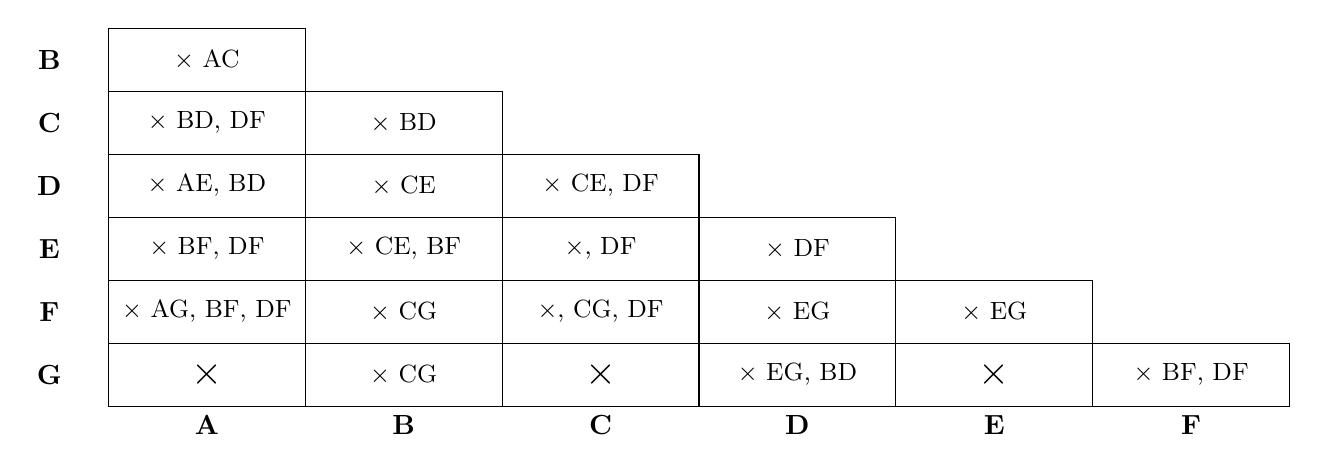
\begin{tikzpicture}[x=2.5cm, y=.8cm, >=Stealth]
        % Draw the grid
        \foreach \i in {0,...,5} {
          \foreach \j in {\i,...,5} {
            \draw (\i, 5-\j) rectangle (\i+1, 5-\j+1);
          }
        }

        % Labels
        \node[font=\bfseries] at (0.5, -.3) {A};
        \node[font=\bfseries] at (1.5, -.3) {B};
        \node[font=\bfseries] at (2.5, -.3) {C};
        \node[font=\bfseries] at (3.5, -.3) {D};
        \node[font=\bfseries] at (4.5, -.3) {E};
        \node[font=\bfseries] at (5.5, -.3) {F};

        \node[font=\bfseries] at (-0.3, 5.5) {B};
        \node[font=\bfseries] at (-0.3, 4.5) {C};
        \node[font=\bfseries] at (-0.3, 3.5) {D};
        \node[font=\bfseries] at (-0.3, 2.5) {E};
        \node[font=\bfseries] at (-0.3, 1.5) {F};
        \node[font=\bfseries] at (-0.3, 0.5) {G};

        % Contents
        \node[align=center, font=\small] at (0.5, 5.5) {$\times$ AC}; % A,B
        \node[align=center, font=\small] at (0.5, 4.5) {$\times$ BD, DF}; % A,C
        \node[align=center, font=\small] at (0.5, 3.5) {$\times$ AE, BD}; % A,D
        \node[align=center, font=\small] at (0.5, 2.5) {$\times$ BF, DF}; % A,E
        \node[align=center, font=\small] at (0.5, 1.5) {$\times$ AG, BF, DF}; % A,F
        \node[align=center, font=\Large] at (0.5, 0.5) {$\times$}; % A,G

        \node[align=center, font=\small] at (1.5, 4.5) {$\times$ BD}; % B,C
        \node[align=center, font=\small] at (1.5, 3.5) {$\times$ CE}; % B,D
        \node[align=center, font=\small] at (1.5, 2.5) {$\times$ CE, BF}; % B,E
        \node[align=center, font=\small] at (1.5, 1.5) {$\times$ CG}; % B,F
        \node[align=center, font=\small] at (1.5, 0.5) {$\times$ CG}; % B,G

        \node[align=center, font=\small] at (2.5, 3.5) {$\times$ CE, DF}; % C,D
        \node[align=center, font=\small] at (2.5, 2.5) {$\times$, DF}; % C,E
        \node[align=center, font=\small] at (2.5, 1.5) {$\times$, CG, DF}; % C,F
        \node[align=center, font=\Large] at (2.5, 0.5) {$\times$}; % C,G

        \node[align=center, font=\small] at (3.5, 2.5) {$\times$ DF}; % D,E
        \node[align=center, font=\small] at (3.5, 1.5) {$\times$ EG}; % D,F
        \node[align=center, font=\small] at (3.5, 0.5) {$\times$ EG, BD}; % D,G

        \node[align=center, font=\small] at (4.5, 1.5) {$\times$ EG}; % E,F
        \node[align=center, font=\Large] at (4.5, 0.5) {$\times$}; % E,G

        \node[align=center, font=\small] at (5.5, 0.5) {$\times$ BF, DF}; % F,G

      \end{tikzpicture}
    }

    All states are incompatable with each other
  \end{center}

\end{tcolorbox}
\section{Race free state assignment}
\begin{tcolorbox}
  If we assign binary state to 7 existing state, it will always result in a race

  \vspace{1em}
  \begin{minipage}{.21\textwidth}
    \resizebox{\linewidth}{!}{
      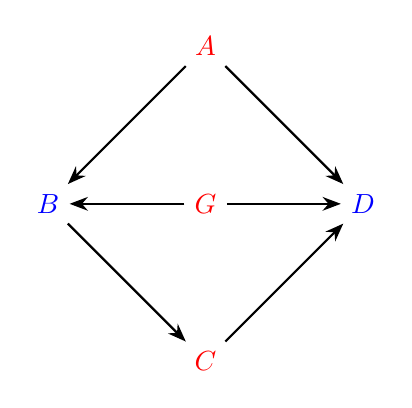
\begin{tikzpicture}[>=Stealth, thick]
        % Nodes
        \node [red]  (A) at (0, 0)    {$A$};
        \node [blue] (B) at (-2, -2){$B$};
        \node [blue] (D) at (2, -2) {$D$};
        \node [red]  (C) at (0, -4) {$C$};
        \node [red]  (G) at (0, -2) {$G$};

        % Edges
        \draw[->] (A) -- (B);
        \draw[->] (A) -- (D);
        \draw[->] (B) -- (C);
        \draw[->] (C) -- (D);
        \draw[->] (G) -- (B);
        \draw[->] (G) -- (D);

      \end{tikzpicture}
    }
  \end{minipage}
  \begin{minipage}{.78\textwidth}
    This is because for a grey code state assignemt (ie that which produces the single bit transition between states), the states must be connected in such a way that they could be placed in the vertices of hypercube. \textbf{The maximum number of common neighbors for any pair of vertices in a hypercube is 2.} Here, states $B$ and $D$ are connected to \textbf{3} states ($A$, $C$, and $G$), hence states cannot be laid out along a hypercube of any dimension, making such 1-bit change binary state assignment impossible.
  \end{minipage}

  \begin{minipage}{.4\textwidth}
    \begin{center}
      \renewcommand{\arraystretch}{1.3}
      \begin{tabular}{c|c}
        \textbf{State} & \textbf{$S_2S_1S_0$} \\ \hline
        A & 000 \\
        B & 001 \\
        C & 101 \\
        D & 100 \\
        E & 110 \\
        F & 111 \\
        G & 011 \\
      \end{tabular}
    \end{center}

  \end{minipage}
  \hfill
  \begin{minipage}{.5\textwidth}
    \resizebox{\linewidth}{!}{
      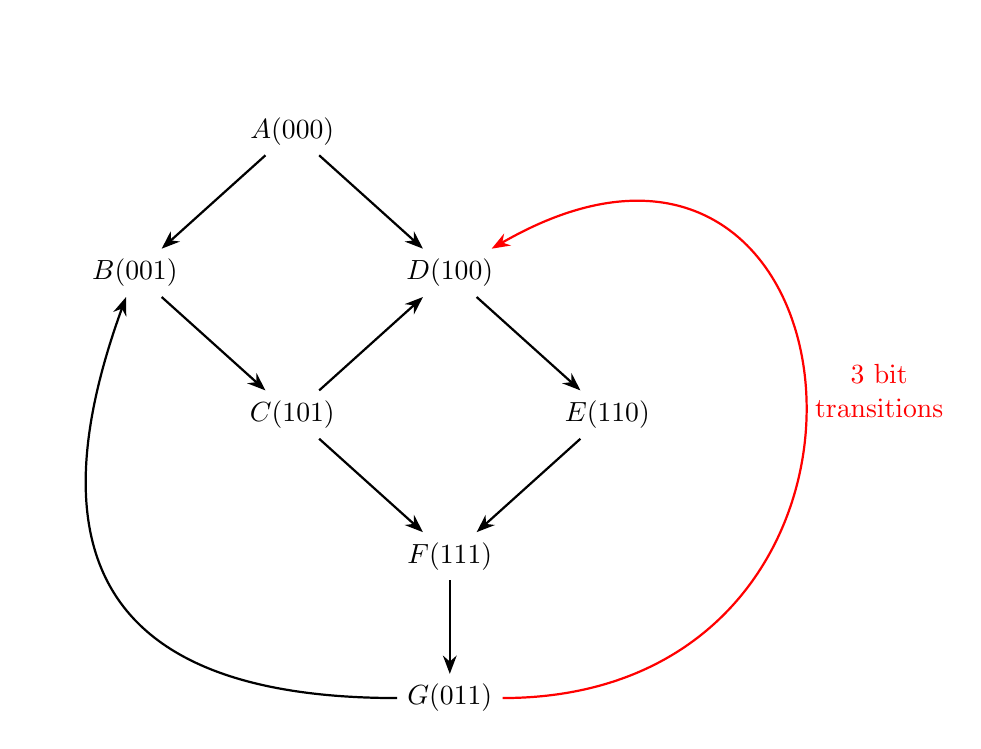
\begin{tikzpicture}[>=Stealth, thick]
        % Nodes
        \node (A) at (0, 0)    {$A(000)$};
        \node (B) at (-2, -1.8){$B(001)$};
        \node (D) at (2, -1.8) {$D(100)$};
        \node (C) at (0, -3.6) {$C(101)$};
        \node (E) at (4, -3.6) {$E(110)$};
        \node (F) at (2, -5.4) {$F(111)$};
        \node (G) at (2, -7.2) {$G(011)$};

        % Edges
        \draw[->] (A) -- (B);
        \draw[->] (A) -- (D);
        \draw[->] (B) -- (C);
        \draw[->] (C) -- (D);
        \draw[->] (C) -- (F);
        \draw[->] (D) -- (E);
        \draw[->] (E) -- (F);
        \draw[->] (F) -- (G);

        % Curved lines
        \draw[->] (G) to[out=180, in=250, looseness=1.5] (B);
        \draw[->, red] (G) to[out=0, in=390, looseness=2.5] node[align=center, right] {3 bit \\ transitions} (D);
      \end{tikzpicture}
    }
  \end{minipage}

  \vspace{1em}
  As you can see $G \rightarrow D$ transition results in multiple bit change.
  Hence additional state has to be added or existing states has to be split.

\end{tcolorbox}
To obtain race free assignment, state $D$ is split to $D_1$ and $D_2$ in following manner:

\begin{center}
  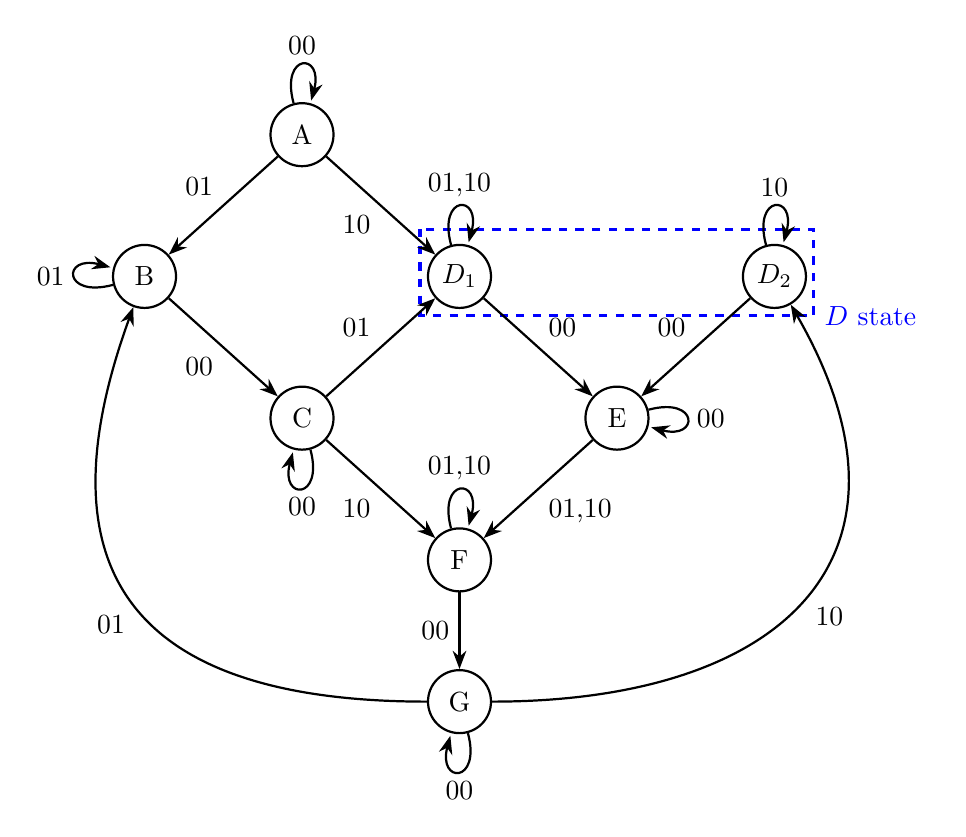
\begin{tikzpicture}[>=Stealth, thick,
    state/.style={circle, draw, minimum size=0.8cm, inner sep=2pt}]
    % Nodes
    \node[state] (A) at (0, 0) {A};
    \node[state] (B) at (-2, -1.8) {B};
    \node[state] (D1) at (2, -1.8) {$D_1$};
    \node[state] (D2) at (6, -1.8) {$D_2$};
    \node[state] (C) at (0, -3.6) {C};
    \node[state] (E) at (4, -3.6) {E};
    \node[state] (F) at (2, -5.4) {F};
    \node[state] (G) at (2, -7.2) {G};

    \draw[dashed, blue, very thick] (1.5, -1.2) rectangle (6.5, -2.3) node[right] {$D$ state};
    % Loops
    \path[->] (A) edge [loop above] node {00} (A);
    \path[->] (B) edge [loop left] node {01} (B);
    \path[->] (D1) edge [loop above] node {01,10} (D1);
    \path[->] (D2) edge [loop above] node {10} (D2);
    \path[->] (C) edge [loop below] node {00} (C);
    \path[->] (E) edge [loop right] node {00} (E);
    \path[->] (F) edge [loop above] node {01,10} (F);
    \path[->] (G) edge [loop below] node {00} (G);

    % Edges
    \draw[->] (A) -- node[above left] {01} (B);
    \draw[->] (A) -- node[below left] {10} (D1);
    \draw[->] (B) -- node[below left] {00} (C);
    \draw[->] (C) -- node[above left] {01} (D1);
    \draw[->] (C) -- node[below left] {10} (F);
    \draw[->] (D1) -- node[above right] {00} (E);
    \draw[->] (D2) -- node[above left] {00} (E);
    \draw[->] (E) -- node[below right] {01,10} (F);
    \draw[->] (F) -- node[left] {00} (G);

    % Curved lines
    \draw[->] (G) to[out=180, in=250, looseness=1.5] node[below left] {01} (B);
    \draw[->] (G) to[out=0, in=300, looseness=1.5] node[below right] {10} (D2);
  \end{tikzpicture}
\end{center}

The meaning of the states are not changed that much.  $D_1$ and $D_2$ now still refers to "balance is going to be 10". But in case of $D_2$ the state doesnt have to handle input sequence $X_2X_1=01$ (\rupee 5 is being inserted) as \rupee 5 can never be simultaneously inserted while \rupee 10 is being inserted.
Hence we obtain following \textbf{modified flow table}
\begin{center}
  \renewcommand{\arraystretch}{1.3}
  \begin{tabular}{|c|c|c|c|c|}
    \hline
    \textbf{Present State} & \multicolumn{4}{c|}{\textbf{Input $X_2X_1$}} \\ \cline{2-5}
    & \textbf{00} & \textbf{01} & \textbf{10} & \textbf{11} \\ \hline
    A & A, 0 & B, \_ & $D_1$, \_   & \_,\_ \\ \hline
    B & C, \_ & B, 0 & \_, \_ & \_,\_ \\ \hline
    C & C, 0 & $D_1$, \_ & F, \_   & \_,\_ \\ \hline
    $D_1$ & E, \_ & $D_1$, 0 & $D_1$, 0   & \_,\_ \\ \hline
    $D_2$ & E, \_ & \_,\_ & $D_2$, 0   & \_,\_ \\ \hline
    E & E, 0 & F, \_ & F, \_   & \_,\_ \\ \hline
    F & G, \_ & F, 0 & F, 0   & \_,\_ \\ \hline
    G & G, 1 & B, \_ & $D_2$, \_   & \_,\_ \\ \hline
  \end{tabular}
\end{center}

From this following following binary assignment is race free:

\vspace{1em}

\begin{minipage}{.4\textwidth}
  \begin{center}
    \renewcommand{\arraystretch}{1.3}
    \begin{tabular}{c|c}
      \textbf{State} & \textbf{$S_2S_1S_0$} \\ \hline
      A & 000 \\
      B & 001 \\
      C & 011 \\
      $D_1$ & 010 \\
      $D_2$ & 100 \\
      E & 110 \\
      F & 111 \\
      G & 101 \\
    \end{tabular}
  \end{center}
\end{minipage}
\hfill
\begin{minipage}{.5\textwidth}
  \resizebox{\linewidth}{!}{
    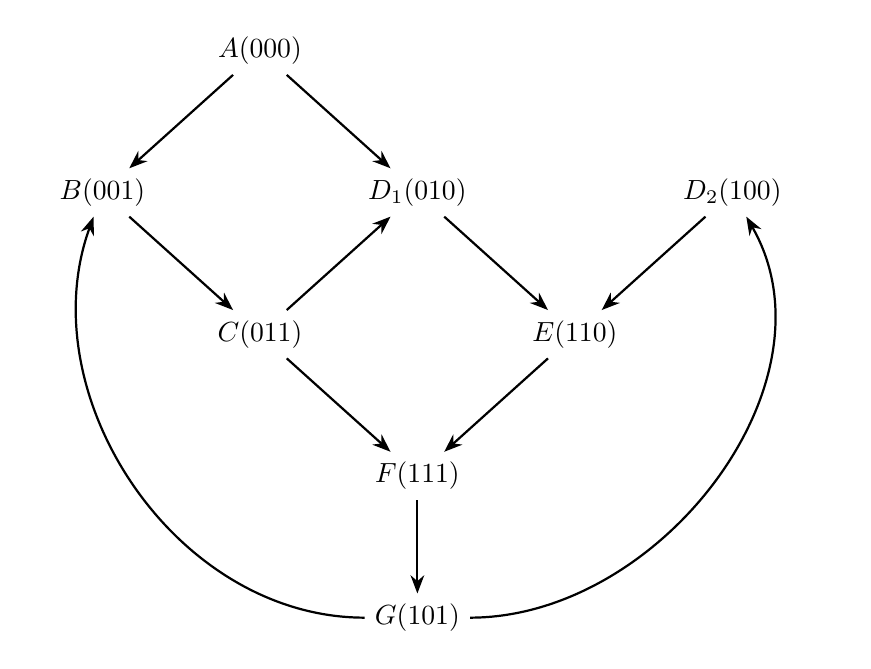
\begin{tikzpicture}[>=Stealth, thick]
      % Nodes
      \node (A) at (0, 0)    {$A(000)$};
      \node (B) at (-2, -1.8){$B(001)$};
      \node (C) at (0, -3.6) {$C(011)$};
      \node (D1) at (2, -1.8) {$D_1(010)$};
      \node (D2) at (6, -1.8) {$D_2(100)$};
      \node (E) at (4, -3.6) {$E(110)$};
      \node (F) at (2, -5.4) {$F(111)$};
      \node (G) at (2, -7.2) {$G(101)$};

      % Edges
      \draw[->] (A) -- (B);
      \draw[->] (A) -- (D1);
      \draw[->] (B) -- (C);
      \draw[->] (C) -- (D1);
      \draw[->] (C) -- (F);
      \draw[->] (D1) -- (E);
      \draw[->] (D2) -- (E);
      \draw[->] (E) -- (F);
      \draw[->] (F) -- (G);

      % Curved lines
      \draw[->] (G) to[out=180, in=250, looseness=1] (B);
      \draw[->] (G) to[out=0, in=300, looseness=1] (D2);
    \end{tikzpicture}
  }
\end{minipage}

\section{State transition table}
The entries are rearranged to make picking the values for k-map easier
\begin{center}
  \renewcommand{\arraystretch}{1.3}
  \begin{tabular}{|c|c|c|c|c|}
    \hline
    \textbf{$S_2S_1S_0$} & \multicolumn{4}{c|}{\textbf{Input $X_2X_1$}} \\ \cline{2-5}
    & \textbf{00} & \textbf{01} & \textbf{11} & \textbf{10} \\ \hline
    000 & 000 & 001 & \_\_\_ & 010    \\ \hline
    001 & 011 & 001 & \_\_\_ & \_\_\_ \\ \hline
    011 & 011 & 010 & \_\_\_ & 111    \\ \hline
    010 & 110 & 010 & \_\_\_ & 010    \\ \hline
    100 & 110 & \_\_\_ & \_\_\_ & 100    \\ \hline
    101 & 101 & 001 & \_\_\_ & 100    \\ \hline
    111 & 101 & 111 & \_\_\_ & 111    \\ \hline
    110 & 110 & 111 & \_\_\_ & 111    \\ \hline
  \end{tabular}
\end{center}
\section{K-Maps for Next State variables}

\def\drawkmapskeleton{
  \draw[step=1cm, black] (0,0) grid (4,4);
  \draw[black] (0, 4) -- +(-1, +1);
  \foreach \x/\lbl in {0.5/00, 1.5/01, 2.5/11, 3.5/10} {
    \node at (\x, 4.3) {\lbl};
  }
  \node at (0, 4.8) {$X_2 X_1$};
  \foreach \y/\lbl in {3.5/00, 2.5/01, 1.5/11, 0.5/10} {
    \node at (-0.4, \y) {\lbl};
  }
  \node at (-1, 4.2) {$S_1 S_0$};
}

\newcommand{\xab}{\overline{X_1}}
\newcommand{\xbb}{\overline{X_2}}
\newcommand{\sab}{\overline{S_0}}
\newcommand{\sbb}{\overline{S_1}}
\newcommand{\scb}{\overline{S_2}}

% K-map for S2
\begin{center}
  \textbf{K-map for $S_2'$}:
  \vspace{1em}

  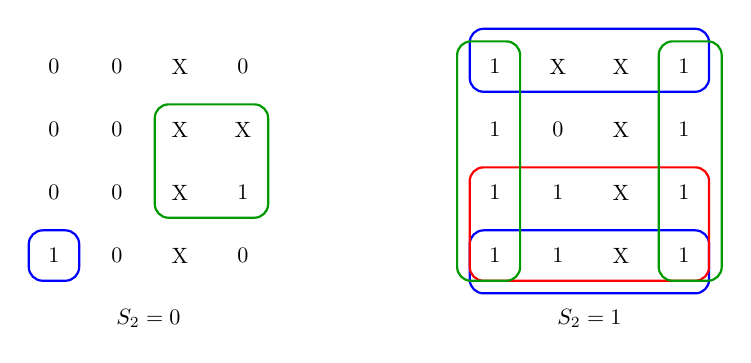
\begin{tikzpicture}[scale=0.8, every node/.style={transform shape}]
    \begin{scope}
      \drawkmapskeleton
      \node at (2, -0.5) {\textbf{$S_2=0$}};
      % Values S2=0
      \node at (0.5,3.5) {0}; \node at (1.5,3.5) {0}; \node at (2.5,3.5) {X}; \node at (3.5,3.5) {0};
      \node at (0.5,2.5) {0}; \node at (1.5,2.5) {0}; \node at (2.5,2.5) {X}; \node at (3.5,2.5) {X};
      \node at (0.5,1.5) {0}; \node at (1.5,1.5) {0}; \node at (2.5,1.5) {X}; \node at (3.5,1.5) {1};
      \node at (0.5,0.5) {1}; \node at (1.5,0.5) {0}; \node at (2.5,0.5) {X}; \node at (3.5,0.5) {0};

      % Groups
      % \overline{S_0} X_2
      \draw[rounded corners=5pt, blue, thick] (0.1, 0.1) rectangle (0.9, 0.9);
      % S_0 \overline{X_1}
      \draw[rounded corners=5pt, green!60!black, thick] (2.1, 1.1) rectangle (3.9, 2.9);
    \end{scope}

    \begin{scope}[xshift=7cm]
      \drawkmapskeleton
      \node at (2, -0.5) {\textbf{$S_2=1$}};
      % Values S2=1
      \node at (0.5,3.5) {1}; \node at (1.5,3.5) {X}; \node at (2.5,3.5) {X}; \node at (3.5,3.5) {1};
      \node at (0.5,2.5) {1}; \node at (1.5,2.5) {0}; \node at (2.5,2.5) {X}; \node at (3.5,2.5) {1};
      \node at (0.5,1.5) {1}; \node at (1.5,1.5) {1}; \node at (2.5,1.5) {X}; \node at (3.5,1.5) {1};
      \node at (0.5,0.5) {1}; \node at (1.5,0.5) {1}; \node at (2.5,0.5) {X}; \node at (3.5,0.5) {1};

      % Groups
      % \overline{S_0} X_2
      \draw[rounded corners=5pt, blue, thick] (0.1, -0.1) rectangle (3.9, 0.9);
      \draw[rounded corners=5pt, blue, thick] (0.1, 3.1) rectangle (3.9, 4.1);

      \draw[rounded corners=5pt, red, thick] (0.1, 0.1) rectangle (3.9, 1.9);
      % S_0 \overline{X_1}
      \draw[rounded corners=5pt, green!60!black, thick] (-0.1, 0.1) rectangle (0.9, 3.9);
      \draw[rounded corners=5pt, green!60!black, thick] (3.1, 0.1) rectangle (4.1, 3.9);
    \end{scope}
  \end{tikzpicture}

  \vspace{1em}
  $S_2' = \scb(\textcolor{blue}{S_1\sab\xbb\xab} + \textcolor{green!60!black}{S_0X_2}) + S_2(\textcolor{red}{S_1} + \textcolor{green!60!black}{\xab} + \textcolor{blue}{\sab})$

\end{center}
\vspace{1em}

% K-map for S1
\begin{center}
  \textbf{K-map for $S_1'$}:
  \vspace{1em}

  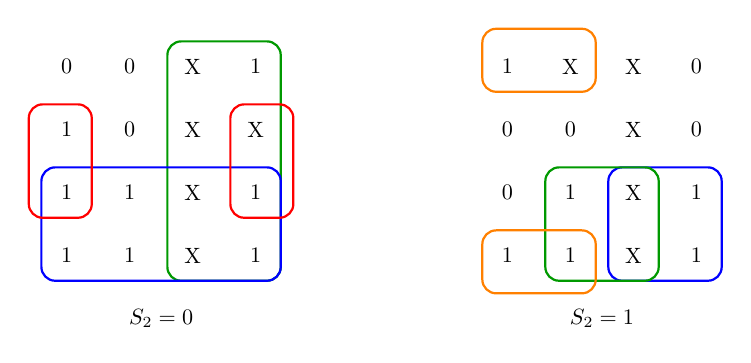
\begin{tikzpicture}[scale=0.8, every node/.style={transform shape}]
    \begin{scope}
      \drawkmapskeleton
      \node at (2, -0.5) {\textbf{$S_2=0$}};
      % Values S2=0
      \node at (0.5,3.5) {0}; \node at (1.5,3.5) {0}; \node at (2.5,3.5) {X}; \node at (3.5,3.5) {1};
      \node at (0.5,2.5) {1}; \node at (1.5,2.5) {0}; \node at (2.5,2.5) {X}; \node at (3.5,2.5) {X};
      \node at (0.5,1.5) {1}; \node at (1.5,1.5) {1}; \node at (2.5,1.5) {X}; \node at (3.5,1.5) {1};
      \node at (0.5,0.5) {1}; \node at (1.5,0.5) {1}; \node at (2.5,0.5) {X}; \node at (3.5,0.5) {1};
      \draw[rounded corners=5pt, green!60!black, thick] (2.1, 0.1) rectangle (3.9, 3.9);
      \draw[rounded corners=5pt, blue, thick] (0.1, 0.1) rectangle (3.9, 1.9);
      \draw[rounded corners=5pt, red, thick] (-0.1, 1.1) rectangle (0.9, 2.9);
      \draw[rounded corners=5pt, red, thick] (3.1, 1.1) rectangle (4.1, 2.9);
    \end{scope}

    \begin{scope}[xshift=7cm]
      \drawkmapskeleton
      \node at (2, -0.5) {\textbf{$S_2=1$}};
      % Values S2=1
      \node at (0.5,3.5) {1}; \node at (1.5,3.5) {X}; \node at (2.5,3.5) {X}; \node at (3.5,3.5) {0};
      \node at (0.5,2.5) {0}; \node at (1.5,2.5) {0}; \node at (2.5,2.5) {X}; \node at (3.5,2.5) {0};
      \node at (0.5,1.5) {0}; \node at (1.5,1.5) {1}; \node at (2.5,1.5) {X}; \node at (3.5,1.5) {1};
      \node at (0.5,0.5) {1}; \node at (1.5,0.5) {1}; \node at (2.5,0.5) {X}; \node at (3.5,0.5) {1};

      % Groups
      \draw[rounded corners=5pt, blue, thick] (2.1, 0.1) rectangle (3.9, 1.9);
      \draw[rounded corners=5pt, green!60!black, thick] (1.1, 0.1) rectangle (2.9, 1.9);
      \draw[rounded corners=5pt, orange, thick] (0.1, -0.1) rectangle (1.9, 0.9);
      \draw[rounded corners=5pt, orange, thick] (0.1, 3.1) rectangle (1.9, 4.1);

    \end{scope}
  \end{tikzpicture}

  \vspace{1em}
  $S_1' =
  \scb(\textcolor{red}{S_0\xab}
    + \textcolor{blue}{S_1}
  + \textcolor{green!60!black}{X_2})
  + S_2(\textcolor{orange}{\sab\xbb}
    + \textcolor{green!60!black}{S_1X_1}
    + \textcolor{blue}{S_1X_2}
  )$
\end{center}
\vspace{1em}

\begin{center}
  \textbf{K-map for $S_0'$}:
  \vspace{1em}

  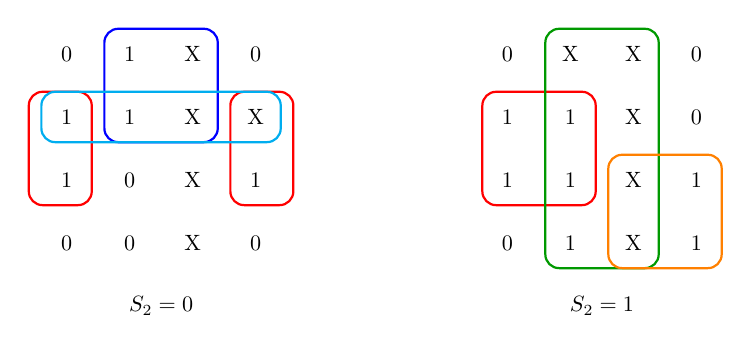
\begin{tikzpicture}[scale=0.8, every node/.style={transform shape}]
    \begin{scope}
      \drawkmapskeleton
      \node at (2, -0.5) {\textbf{$S_2=0$}};
      % Values S2=0
      \node at (0.5,3.5) {0}; \node at (1.5,3.5) {1}; \node at (2.5,3.5) {X}; \node at (3.5,3.5) {0};
      \node at (0.5,2.5) {1}; \node at (1.5,2.5) {1}; \node at (2.5,2.5) {X}; \node at (3.5,2.5) {X};
      \node at (0.5,1.5) {1}; \node at (1.5,1.5) {0}; \node at (2.5,1.5) {X}; \node at (3.5,1.5) {1};
      \node at (0.5,0.5) {0}; \node at (1.5,0.5) {0}; \node at (2.5,0.5) {X}; \node at (3.5,0.5) {0};

      % Groups
      % S0 \X1'
      \draw[rounded corners=5pt, red, thick] (-0.1, 1.1) rectangle (0.9, 2.9);
      \draw[rounded corners=5pt, red, thick] (3.1, 1.1) rectangle (4.1, 2.9);
      \draw[rounded corners=5pt, blue, thick] (1.1, 2.1) rectangle (2.9, 3.9);
      \draw[rounded corners=5pt, cyan, thick] (0.1, 2.1) rectangle (3.9, 2.9);
    \end{scope}

    \begin{scope}[xshift=7cm]
      \drawkmapskeleton
      \node at (2, -0.5) {\textbf{$S_2=1$}};
      % Values S2=1
      \node at (0.5,3.5) {0}; \node at (1.5,3.5) {X}; \node at (2.5,3.5) {X}; \node at (3.5,3.5) {0};
      \node at (0.5,2.5) {1}; \node at (1.5,2.5) {1}; \node at (2.5,2.5) {X}; \node at (3.5,2.5) {0};
      \node at (0.5,1.5) {1}; \node at (1.5,1.5) {1}; \node at (2.5,1.5) {X}; \node at (3.5,1.5) {1};
      \node at (0.5,0.5) {0}; \node at (1.5,0.5) {1}; \node at (2.5,0.5) {X}; \node at (3.5,0.5) {1};

      % Groups
      \draw[rounded corners=5pt, red, thick] (0.1, 1.1) rectangle (1.9, 2.9);
      \draw[rounded corners=5pt, green!60!black, thick] (1.1, 0.1) rectangle (2.9, 3.9);
      \draw[rounded corners=5pt, orange, thick] (2.1, 0.1) rectangle (3.9, 1.9);
    \end{scope}
  \end{tikzpicture}

  \vspace{1em}
  $S_0' = \scb(\textcolor{red}{S_0\xab}
    + \textcolor{blue}{\sbb X_1}
    + \textcolor{cyan}{\sbb S_0}
  )
  + S_2(\textcolor{red}{S_0\xbb}
    + \textcolor{green!60!black}{X_1}
  + \textcolor{orange}{S_1X_2})$
\end{center}
\textbf{Notice that we have added extra grouping that overlaps with other groups (higlighted in \textcolor{cyan}{cyan} color). These additional groups are necessary to remove hazards in circuit}. Here is a circuit if these groupings are not done: \href{https://www.falstad.com/circuit/circuitjs.html?ctz=CQAgjCAMB0l3BWKtIA4BMaAsBOHqA2dAZlX1QgUhCS2JoFMBaMMAKAGcpx1UQcCPPtQgAXAE4BXBp25gc6foPmKRICdLYAPEMSRgESIuAR8sIdOYAa7HcXPoSIAhEeCH19GwPUEC8FjmAOyQ5mCB3Oa+bACS4P5gvBYIyknUMEgIsfGKKsnK-unQmWwAStyo6bqqkb7cRVkA7hVVicJszdSVcoUdSkI5A5B9AoN5ecPN6CkD6EG5aX1+uQTUxMTKq1B9cyvUu0M7M3kHEzvz4EGCp71xeopM3fcgLIINNNlYYIKP1F8-33qxQ+cQQiRe3TBD0B7yaFgu3zWG3AW0m8NyV10CAxbz6zzAmOWl1xdkBTAu9geBBwIA8IAAyl47KgkOTFF8IExqbSLOZ6bZaRcueZcHwuRA6fS0VCXoCZW1ts15UkiQq0f8IX8sGLuurtZrafrRnq+M9Anxjd4qM40PkQCEHDN9tw4TLfjQIu7pZ7IRFLOkln6sNRVnx-YqbWGLtNrhc0TH0Sj9nG+ojE2mzs0M-5RmcDIornw8qhuhMLC6+g6AsECEWImjC9X7bXiRHG5g+O2nZWWwmqwnhvnI7oW1WNsJdDQPkqEuDzeBwSaF+z9V6luCFTLxxH8VtnqQonjsbpUCLiIoDzvj2n1psA81589Q1jVOuLy3n9v1eeT+ZP6fth8fhMQJZRIARTFnWiICcExfFwIvY9nRKZoSxEHMIkze1QhHC0Ii-I9oUEfdX2aEiQDIYjSIo0Yf0opMI3otMcEw1FCINZ4WHrdiuPMHBwV4iMWLCLZYLvISQIwsJemaYTcOA4iWzRfjoQiBQxXCQ9ZKSQT1N0ZFlKSW8FP03Eh1YTA7USQEB3LFDwAQ1sLP2YMI2c9NHOeNFrOuY50DJTS3P8gE1IEwLB2tZ8ZSrGVkOnYdcGI49EqvdlaOPS80SilUImxdolVynKPADIcgmPGVTz4WLJ3stNTi2FJ7wY+cypXfLDSqrZWpoNiH31RqOpfQDIttAgZirMa3knaJmmfAhXKfVy0UWtZkstWbRpmYzJp3ZEduM0DduUTFTkgt95JlAgUyVcErsUOaUyA59uqrbqoPi+cBpagy+m+wRnp+jbOxbBVG28pJGwVNVUySBVc0WJ7bUq7DzGR964WfVAf3nLHqJx7H9SCQGGORtMBu8rZ5zqx7jyrSoujgCjGfRyscJetmAIbHCKEEOn9WGHR5noMqIAwJAypFCxqH5GwAB0AAcZa8IGKPmkm1Ypro1bTNGrQLD8LmRu7uBqOFuoG83FmaGLwXNxdKzW3nkv5ns+B2ibu2t49a07WnLIbUdLPp+1-b6YP5gZyO3MSXwEkcnbvMclL3PJq1qDE5xjnjp07I+GDMWTpPjXLaDrxjmgQOCiuptNkYjORPT5qaxvXIzpuJP+w39WNtFkZlDPYpGAvuno7UmtHkfczYnQxppKhxZVW1JUgGwACM0+HOSqzklmVYEEQkn3oKLS2UGlL15sLSSQg+LSXOzZbLecJ31nzGinCiS5t--BvmgZNV7+ihf660RkWSA40cJgHATXKcrpCpVUwqEJqCBEGuWfFApafR0GeWRFA66pkHIUj2p7JmUdg6-wbMiYBjMKEX0hkggBDklr31dg5CBYRoFthBpASw9pcE8K0nwsCvCiaCFodbFs9FGxoS4XwGRwDdRhzVvI5RLsJFuxLPab2miGx+2oI2COsiaK80fvbcyYAG6YRIIoHeJc87WjwDYjcaALSLjsVkGCcdeFQM0VA3hcU4Q+NcbkCxgg9LeVCUoEQLiHL+KURw1ucdMGoTVnpRx-Ara0gCu4QEKkIwakbracJv1clzlyZklu6dYZwHanpKBRS462mUj-UY9F6K91aZ09wiisxVwQJXNW-TcS9MGQM8wLB7YjPGRZLJAJJmzNlGUn4PSPTjNLOgUYa5embPWaMF+2ywlWJ-C-ICQSFwg0wCIb4E56D2U4oFYgOFBLLSeQ8j+Z0yLvOIpAocLywjmRiawJCJSwlJA1Kwc+WZAXXIWRC9qZzWAARQf8zmgYUVv1QU1Hy5yiyXJxdsIAA}{Click here}. Notice that circuit oscillates by default. It will also oscillate if you switch $X_1$.
\section{Output expression}
Since output $z=1$ only when current state is $G$, so a separate "output transition table" is not drawn. We can directly write (from binary assignmet for $G$) that:
$$z = S_2\overline{S_1}S_0$$

\section{Circuit}

\href{https://www.falstad.com/circuit/circuitjs.html?ctz=DwYwlgTgBAZgvAIgIwKgFwM6IAwDpsEECsqYIiSuAHACwDsAnEVQGzYtIENVEuogAjCqgAOQhDQDMqAG4REJKAFtMCgKYBaJCgB8AKChRgGKAA8cUJACYqUBi0s3U8BNlHDlSxGggBXNQgA9PqGxmYWSAxWdg6RVs447sioSl4IPv5BIUam4QiSRJZEhSzRSMwJEqgYYIhWNKhoaogAGijBBjl5kjRQVlaSUBx9VnywiA1QNXWTTa3xHaEAggB2ACZ5RFGWNL102L1Iu5VuUGArE1mdwACSeXGOtla8jyfVADY4uIoAFrUIJEWRju5mQ2wez1iUTeU0+rm+qD+CiuoQASnlsFAqJjMZJ4uNXKgAO4uU5KACGphkyKBt26RGiGmxUAKjKQY1JHy+v3+gOydNBNHZUCZmKFDi0HMSsO5iN5KOBm2sIuZRGVkphGDheB5NP5uVBkmFGjo0R6jJYDEqk2mCHqjWaCAAygt9d0eCLTVAhUgRZbrdV-vb0I6ne03YKvRoWL0aNw-SgCTag7NQ25aasNqC2E8XvtepC3rSAPLQUF0Fi2B5UZlxIv80t5HMsytQfMtqgw86IaRQAD2euumbyDArljHnC9SAr9aH6xHY9ZlmwXtZs9CjdB2ismMhjmFhYJ6f5w+z2Fsaui7cv66Mm8QdAZUEvWJoF+sXYu+QVwFPiGbla2O2gEwgOAI-n+CDNo+V4HG2DK3r+85nrYtBAXBaGIfeCDttimJ4ViBCIQaD4DPBvpUM88GTC4yZ1KcczOkgbQANRhi0rrXNhFa2CwXpoUMpqgYOyzIYgo4OCwLyTtEUlSoSGZiQgEnevYy5enG8nHlxZYUNYmJEBOVjCoZWk-iRUFbM+2CFKaF7ngGUwpg6iBOtgbQCBBSnNlE6G9L5WG6Thra+ViMZ2E4R6kF+0iKVm-7nsueZwZwvCBXkPHLjQ+HhZw2XpVuSCSA4DC7I4eJ2McUVxSO2wMMqnA1nYH7VSeSkMOC2D1MuTWcMGnI1Vu55VuyVY7pi2iVp+PZefFUGJR1sH+dCrXXAA5vcxUTaNlhbY4RGraEAAyACiAAi9yjIcO1FWwlijZU+JKGBaxqDA5K+O8aAaO8ahrPw8jJFAIBrdKgjSkoAjkPC2DhtcFlFdo930Lt-T3UQpy0YGMwuQgABe5n3DQxneocux0N6dCObawaMS6P6nRdW6SGO-Rk16bOPSkL1vR9X0-X9AMeCDYPiGSUNfLDP4bVu9DRGzOwc2lh1dLLZHWIMRxxo48l0XaqauXDx3nZtE5lUcU5VS4T08+9n3fb9-3A4DiYi4SwNiykEsw0bRiM6bkns7JNF1NziCvXb-OO0LQNu6c4Pu5D0N4FLtII8Tgw7oUWsMH0DlJtj+u425P4QESGKEVAE2RZyOjYAANNiADcDfWFQwCBGX-JlxXzITSttcN83rdRB3XfXD3oJqW3ljgjXiQ6PY9dt03cTLzYY9Et35dT1CZTggPC9L3Eq9RMvo+d1vE873U0k2CyxWWGwbw6JC69UE3Vimu-n-f+y2BN0kMVZebBN7b02OCO6QDYjPyijoLYVgQEAOgUgsB188h7ghFOGccC34ny-og-Bf8KxoNCJPOo2CHAIPHGZV+xCWCAIZMvCsTcEHMJYKQow5CATqhMg1eehJ4HWHrpKVhwi26cOANwl8M9qFtxfpeH+bCJGX3AYKY0zJdi2FFC-cUIjm5aP0dgSR3CtEqjFG+FkCE4GGNFE3Qx9h7FvnrqyExN8eGMlVGVHRcDFF2KILsIxbjNjeK8QWfKvjAn+MCfUYxqj0GggCeEzEzZYkKJidlJuOZ66xOCShPoU47oEJftkghn9eA5NNKvNglSrB5IoEUr009D6CP-rU6pI8rBN2PhfceZD3Hti1m2Vs05aH5mXrsJuPEJk0CmZWdh9TgpPESu2Q8tdpk7g-hs3gUyDg5N4IsuRyozE+Nrso6wTiqDLwubY7Ehz+HvjNFNXx4ibBiMQcVdu8T+n0jNLQB+MDMYL1ZC42gjDCFsEAcA-+iylySH+c2eFIdBEgqRfYvEoLZnZKRYssxS5EXWNroY1kWTzwuIZPcp5vFEqfIUcIz5pKrmfMWTWfu0QVJ1jgay8+XTSo0B5d0isPLFntk+XYRczz1l7IZXylxlZBUsDlV8vpXD3FLklFiaesDa4gtEairpVAl54iboaxVMLvmqryKap+mIOXaoXqapB3TAn-wVagi1Ui1VPlFFYtkVtgVMLsbqrWsLvVDPqn65FbgdDBsmRGkRIaPXcIjSKcN99oEv3jVoONNgE05qZcVRZoVoHiocBmuBvkXHFTddAxZMkaH3R3H0CJtcZLsNXvpHJ2U636QKWUFcZpCUL23A3MpbbXFJvcdYA8LwU3ZqjQgHQ07FWQlXsZRV87unCPnYs5smlfWqVodkzS4L66aVDdEfdcLaAvxBSe1FtBd2JQZBeMqL6SlkpfawwJL7Dlvvvkk5tQLBFJPrl+0DuTJ33EabJRKrAF1LpqWOmpvAAFtLQh0xuMZGVYZoCKp8+7-59pfjBM9jjSNaMw5RtpBD8PRBfaTC8OD1lMK-aR1DlywOQsMaZXFljTKMd9bo5xplOMTpVZ6psiU+JmkfiBOB2SZNQsVUplBgFFkEIbSW+TtcCHtpQaM5T9c5JGfU1BxJyoxUvnzHSj58rFFKYc+ed59d8yUrbHBaCBxbOuYODhtz5mJj8bHGYugxVhNXNE4YsLHDAsSEsTFoYKzws2OcTF-zha4vQRGffHiH6rk8TXQVysdbcshViAI6NbdXPyuqyvY+G8stwYqqFlLtdslUGNYYzrXTouZYk9w9sMEPN7BvXA8ZMFdn8roI+uLuFhS4TfCRvZVB2RTcbm+EVcFrNPhvONvZl4pmsesCygghFMSZR0w6ggjcCAmpu6aAB0zHtHcQS90jgE5lXLMwNqdva5EDqGMrVtnaEGrwHcZg5cX62Ef+-a1pEOT0jq43E37I502P1CjGYD0bK3QO6bm7HRb77Y9LUMFtR9CeZIksZ7tcWVIydfLxISFahVKbQsZ00LL+PKhUnt2uHPDs08vEWkLzJrVvhx4umnkuTVL0lyytSkvNWApfo62XjrzVo-yXyx4wzOwKbJXyor9djfVZ4lt3o1mQotSlfyw74ywfwbA1EE1MYNsf2d6yr7jdm7TNNT7iNf6rcAfNgcKX8Cf1vNA3lVHV8fmJLD9lJLVZw-pP5bHnDsen2p9XHJms+Xl4DqMzJUzNZTv4TO5lPqCG8K3YAXX+DUzgFN5i0X+oPua8ipGTZBwgze8kfmalBh4zh91uGs1Mot0IoG9bcNU3FztDAN8j2zHd1Gqp-6sO26pvIUb-b3huL8Gsq2s6hTwRzvM+LSL3T7XiBj+hUWjPtX7vfLdLPivuL4pU0OG-xG3R7ICaDCeiQeX+woKaPktuC8IBFy2SoBd+Eg4BDUE+k0s+0BgBEa9iGBbyeiqB4ONY1yJW9OJOyeT+nA+ctcla2OBOVy5BH81+dBRa2w1qEu2ImaZ8AejqnB8udy0O66z4Rk4UpkL8y6YGLC1g7uvGfBQhIWGiEeEh9u4hV0CaNygBWgqhG6vBCBgGPq1gakpyC8oGdiehmhceaiFAVg+htYAw7K-qrSlhpha6S8ZuNhpuuwF6qaYevU5Q+IOqgaWsgCeym6kgB2LCIRGePh+BtBPh4+3h-ygGseIh8+2gYKMeSAqRLq4epWZ2qBOs10kqw640hBH8oheB1gziZRyhqBludg2wmUfKy2-Ki0UyO4puruj2bhsy0yfKOeZOCRaehuVyEk36TRLCMeWRTWqeiUf+UBgi2SdBWBZqBAH8MBdSc2nmTUl2wOC84yn2uxOy0yckNRoU9RlWi64yb+3RjWCBRUY4uU-Bayw6LMKmsyoh2GohkIdazxOwhwV0AhtCtxZqkyChMya6khJC0O3xCsJh5iIhzxOSHeJhCJrxDhQS0Ocs5OisZQdhVWcstOq8eJiaNxGJQyFs8sW+rShJwJeJbMaCHc4AEA+gQAA}{Click here to see simulation in Falstad \\
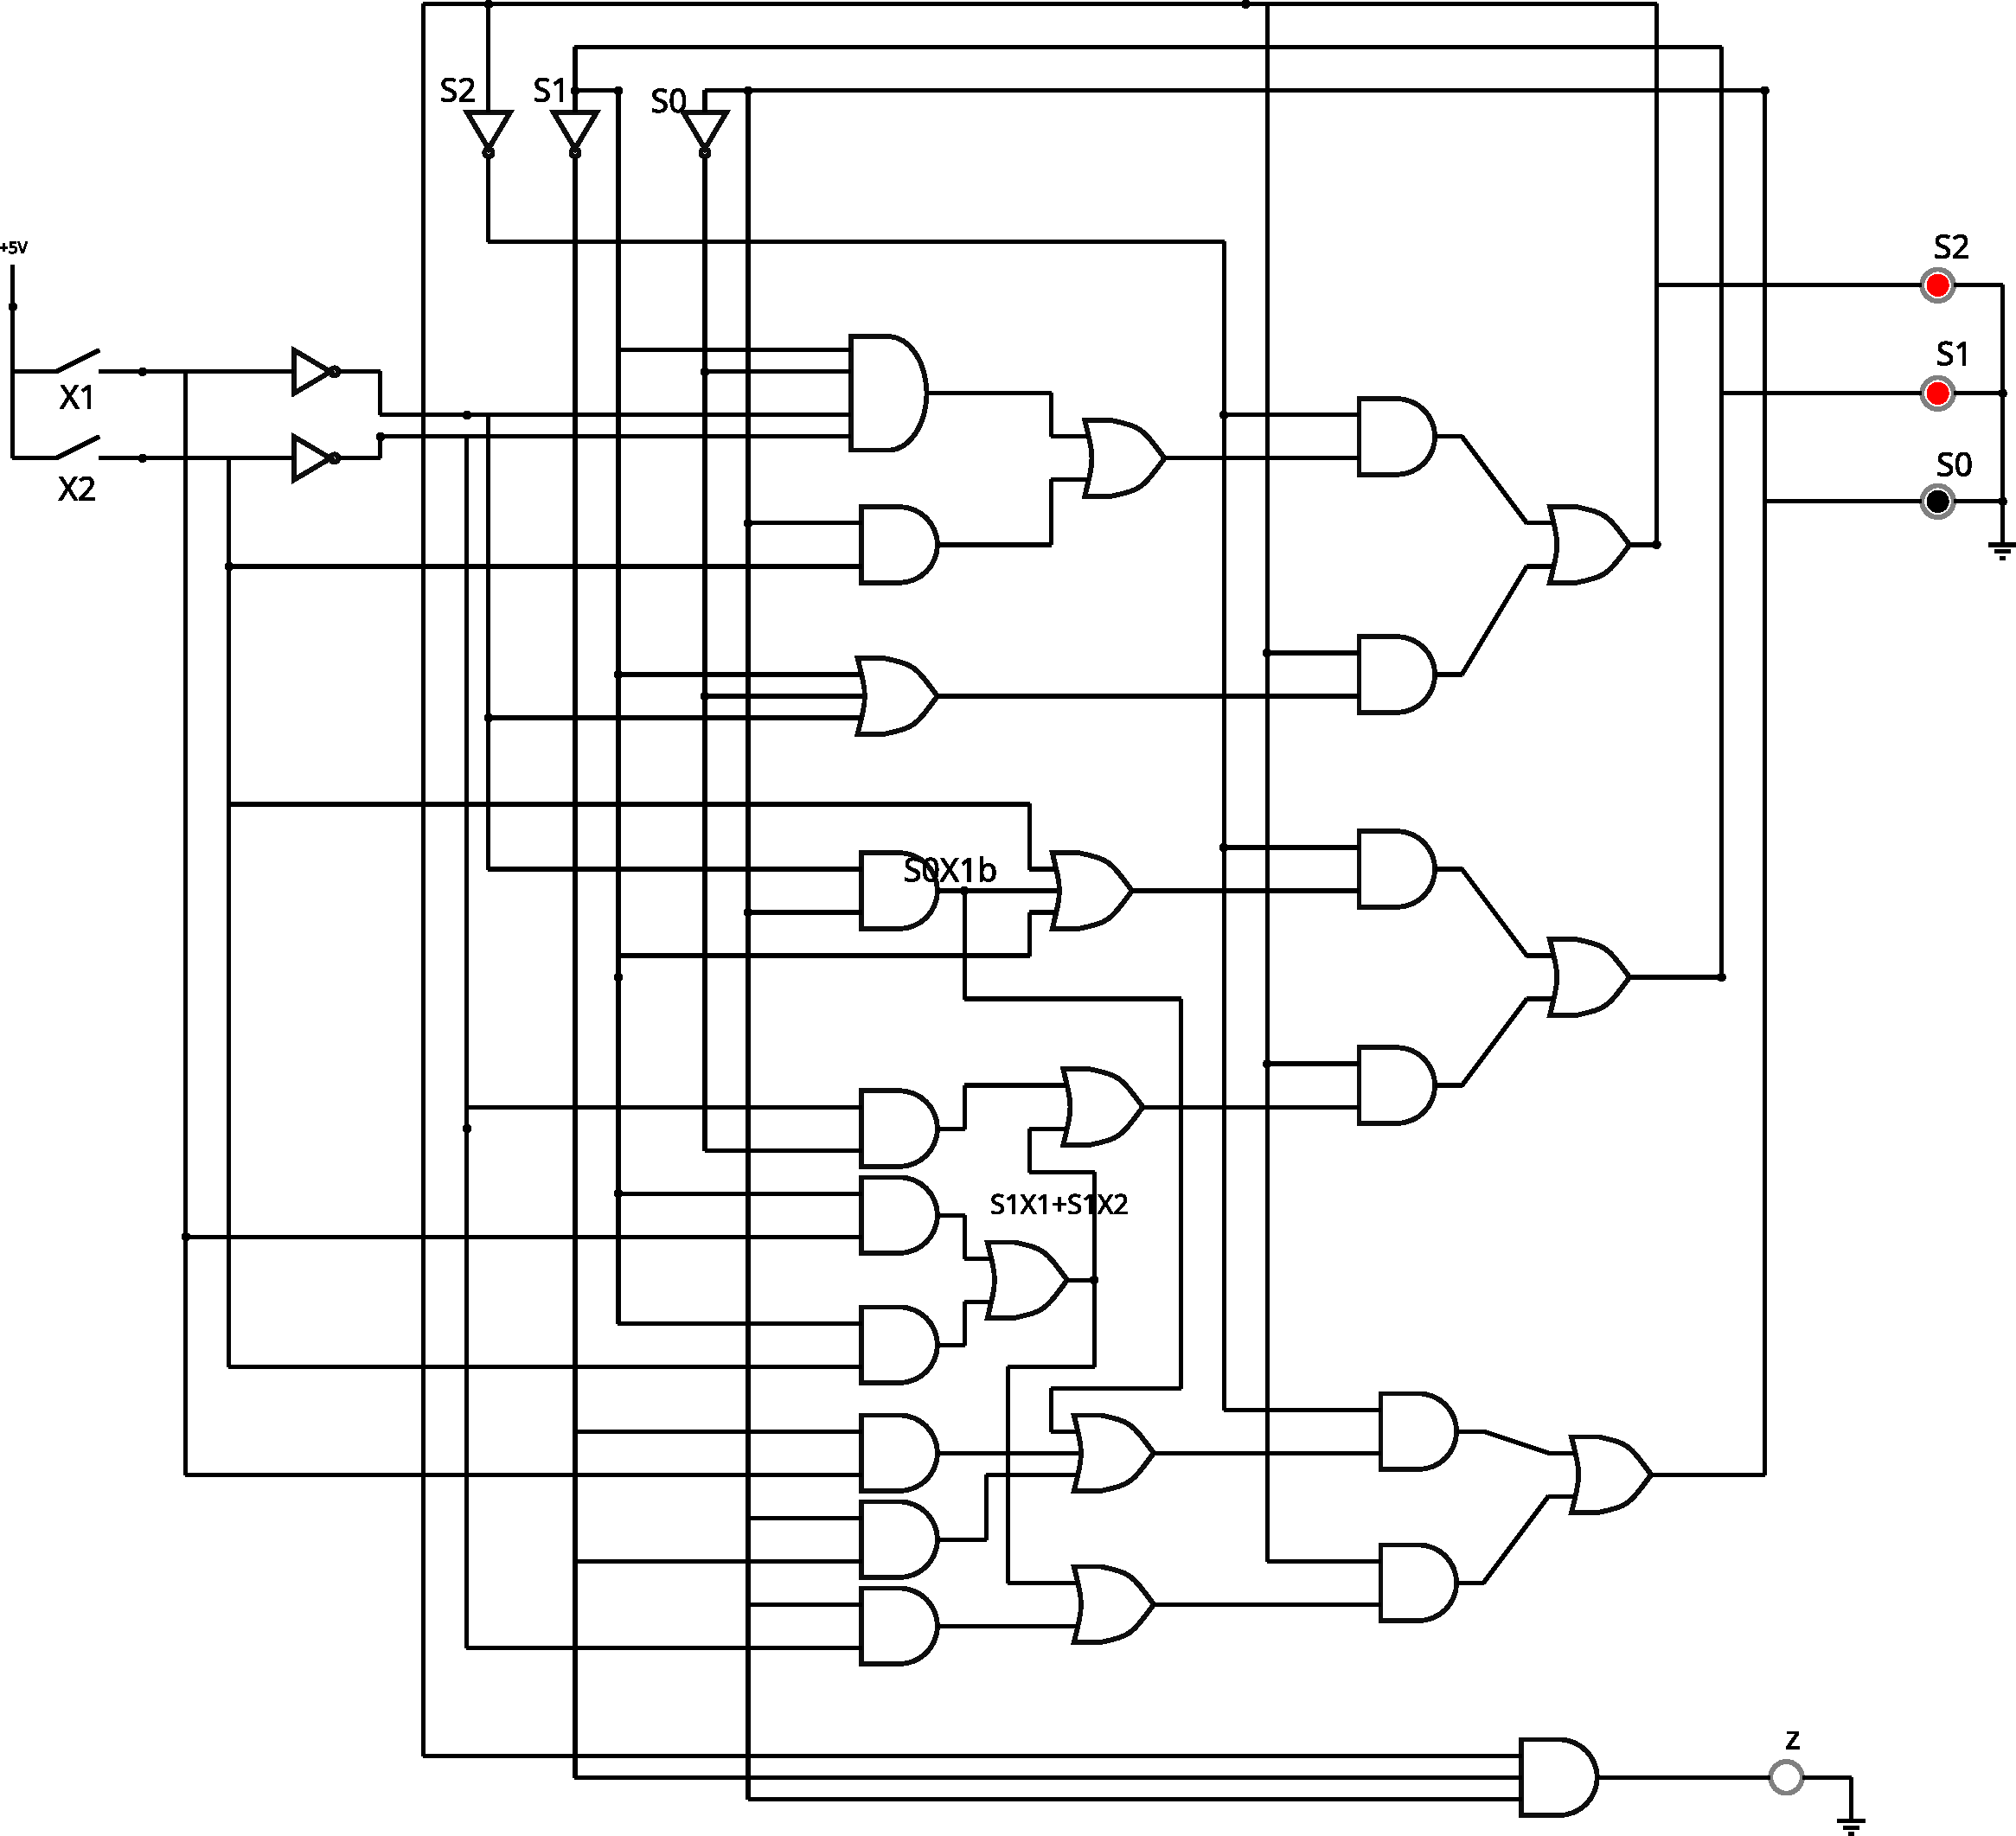
\includegraphics[width=\textwidth]{circuit.pdf}
}

\end{document}
